% In this chapter we will discuss the response of Jupiter's
% magnetosphere and ionosphere to changes in the solar wind
% and IMF. We already have some plots from our paper but we
% could greatly improve upon the analysis. 
% Improvements:
%       1. The response of the magnetosphere needs to be 
%           further analyzed. 
%           - Plot showing how the pressure pulse propagates
%             through the magnetosphere
%           - Analysis of corotation velocity and field aligned
%             currents in the magnetosphere. 
%           - 

\chapter{Response of Jupiter's magnetosphere and ionosphere to changes in the upstream conditions}

\section{Introduction}
The gas giants, Jupiter and Saturn, both possess a strong internal magnetic field like Earth, but the relatively fast planetary rotation and the presence of significant internal sources of plasma lead to vastly different magnetospheric configurations and dynamics compared to the terrestrial magnetosphere \cite{Khurana2004a,Krupp2004DynamicsMagnetosphere}. The internal sources of plasma at the giant planets are supplied predominantly by their moons, Io at Jupiter \cite{Bolton2015a} and Enceladus at Saturn \cite{Blanc2015}. In particular at Jupiter, through ionization of its volcanically erupted neutral particles, Io supplies heavy ions at a rate of $\sim$250–1,000 kg/s to the magnetosphere \cite{Bagenal2011b}. This leads to a high‐density plasma sheet that is forced to corotate with the planet to large radial extents ($\sim$20–30 $R_J$) by the corotation enforcement current system composed of radial currents in the equatorial plane, field‐aligned currents that couple the magnetosphere to the ionosphere and Pedersen currents in the ionosphere \cite{Cowley2003a,Cowley2001a,Hill1979,Hill1980,Hill2001,Vasyliunas1983a}. In studying the complex spatial form and temporal variability of Jovian aurora, it is typically subdivided into three components—main emission (oval), polar emissions, and equatorward emissions. The main oval of the Jovian aurora is thought to be at the location in the ionosphere where upward field‐aligned currents associated with the corotation enforcement current system are present \cite{Cowley2001a,Hill2001,Southwood2001a}. Theoretical models have predicted that a compression of the magnetosphere due to an increase in solar wind dynamic pressure would lead to a reduction of the main auroral oval intensity on the dayside \cite{Cowley2003a,Cowley2007,Southwood2001a}. Subcorotating plasma in the dayside equatorial magnetosphere would speed up in the azimuthal direction as the magnetosphere is compressed due to conservation of angular momentum, thereby decreasing the strength of the corotation enforcement current at this location, which in turn would dim the Jovian main aurora. Using a global magnetohydrodynamic (MHD) model, \citeA{Chane2017a} found that while the nightside/flank currents in the ionosphere are enhanced due to a simulated forward shock, the dayside currents are weakened, which is consistent with the previous theoretical prediction. 

Although the Jovian ultraviolet (UV) aurora is well structured and always present, remote observations made by the Hubble Space Telescope (HST) and Hisaki/EXCEED observations of the Jovian UV aurora have shown that its intensity is highly variable and is often correlated with the dynamic pressure of the upstream solar wind \cite{Clarke2009,Kimura2015,Kimura2018,Kita2016,Nichols2007a,Nichols2017a}. Due to lack of a dedicated solar wind monitor at Jupiter, identifying the correlation between changes in the auroral emissions and upstream parameters typically requires a numerical model, typically a 1‐D MHD model \cite{Tao2005,Zieger2008}, to propagate the solar wind from 1 AU to Jupiter's orbit, which is subject to timing errors due to assumptions made in the model and the orbital geometry/alignment of Jupiter relative to available solar wind monitors at 1 AU. Exceptions to this situation include Cassini's flyby of Jupiter and Juno's approach orbit, during which in situ measurements of the solar wind and remote observations of the Jovian aurora could be made simultaneously \cite{Gurnett2002a,Nichols2007a,Nichols2017a}. \citeA{Gurnett2002a} report an event where Cassini observed an interplanetary shock a few hours prior to a large increase in UV emission intensity from Jupiter. Recently, \cite{Nichols2017a} report observations made by HST during Juno's approach to Jupiter, during which the Juno spacecraft detected a large increase in solar wind dynamic pressure \cite{Wilson2018}, which resulted in intensification of the main emission in UV, observed by both HST and the Hisaki spacecraft \cite{Kimura2017}.

Intensities of the polar emissions are comparable to those of the main emission \cite{Grodent2003a}; however, unlike the main emission, they do not have a steady morphology and are highly variable. UV observations made by HST have shown that the polar aurora contains highly dynamic regions with different repeating patterns such as “swirls” (in the swirl‐region), “arcs,” and “patches” (in the dusk active region) and occasional “filaments” \cite{Bonfond2017,Grodent2015,Grodent2003a,Nichols2009a}. Due to the complex rotationally driven dynamics of the Jovian magnetosphere \cite{Vasyliunas1983a}, it is unclear how much open flux is typically present in the Jovian polar regions, and which features of the polar aurorae map to open field lines in the solar wind as opposed to processes in the outer magnetosphere or magnetotail \cite{Cowley2003a}. Some models argue that Jupiter's magnetosphere is largely closed \cite{McComas2007}, since the reconnected field lines may undergo successive reconnection during the time it takes to travel through the magnetosphere, while other studies predict that Jupiter's magnetosphere does contain appreciable amount of open flux \cite{Cowley2008,Masters2017,Vogt2011a} and that the Dungey cycle \cite{Dungey1961b} and the Vasyliunas cycle coexist to influence the structure and dynamics of Jupiter's magnetosphere. 

In this work we introduce a new MHD model for Jupiter's magnetosphere based on the BATSRUS MHD code \cite{Powell1999a,Gombosi2002b}, which is coupled to the Ridley ionosphere Poisson solver \cite{Ridley2004IonosphericConductance}. Unlike previous MHD models, our model includes mass loading due to Io in a self‐consistent manner at the right location. Using the MHD model, we investigate in detail the time‐dependent global response of the Jovian magnetosphere to different types of solar wind disturbances, such as interplanetary shocks and the rotation of the interplanetary magnetic field (IMF). We analyze the response of the corotation enforcement current system to these upstream changes. Through our model we also identify closed and open field line regions in the northern hemisphere and southern hemisphere of Jupiter to understand the magnetic topology associated with the release of plasmoids and other dynamical processes. 

Following the procedure described above, we have conducted a series of global simulations with different sets of upstream conditions given in Table 1. In this work, we are interested in understanding how the global magnetospheric configuration varies depending on the solar wind and IMF conditions. Therefore, we first run the simulation using fixed nominal solar wind parameters but with two different IMF orientations: Run 1 with a purely southward (parallel to Jupiter's magnetospheric field) IMF to minimize effects of dayside magnetopause reconnection and Run 3, with the IMF in east‐west direction representative of the typical Parker spiral configuration at Jupiter. For each of the two IMF orientations, we perform two additional simulations (Runs 2 and 4) in which we introduce a solar wind dynamic pressure enhancement to study the response of Jupiter's magnetosphere to impact of interplanetary shocks. 

\section{Response of the magnetosphere to variations of the upstream conditions}

After creating the quasi‐steady state magnetosphere using a purely southward IMF, we continue the simulation in time‐accurate mode and perform four simulation runs using the following sets of upstream input: 

\begin{itemize}
    \item Run 1: No change—continued run with fixed southward BZ and steady solar wind
    \item Run 2: Introduce a dynamic pressure enhancement (forward shock) under southward IMF
    \item Run 3: Turn the IMF from a purely southward ($B_Z$) to Parker‐spiral like ($B_Y > 0$).
    \item Run 4: Introduce a dynamic pressure enhancement (forward shock) under Parker spiral IMF
\end{itemize}

Two configurations of the magnetosphere were first created: Run 1 for a closed magnetosphere a parallel/southward IMF and Run 3 for an open magnetosphere with a Parker spiral IMF. After the completion of Runs 1 and 3, upstream solar wind conditions were changed to simulate a dynamic pressure enhancement similar to that expected for an interplanetary forward shock (Runs 2 and 4). Solar wind plasma properties and magnetic field magnitude between Runs 1 and 3 were kept the same, that is, same mass density, velocity, and thus dynamic pressure. Likewise, the plasma properties and magnetic field magnitude of the shocked solar wind in Runs 2 and 4 were kept the same, with the only difference being the IMF clock angle. We designed these simulations specifically for understanding the influence of the solar wind dynamic pressure enhancement on Jupiter's magnetosphere under two different states: a closed magnetosphere with minimal impact from dayside reconnection and an open magnetosphere with dayside reconnection expected between the Parker spiral like IMF and the magnetospheric field.

\begin{figure}
    \centering
    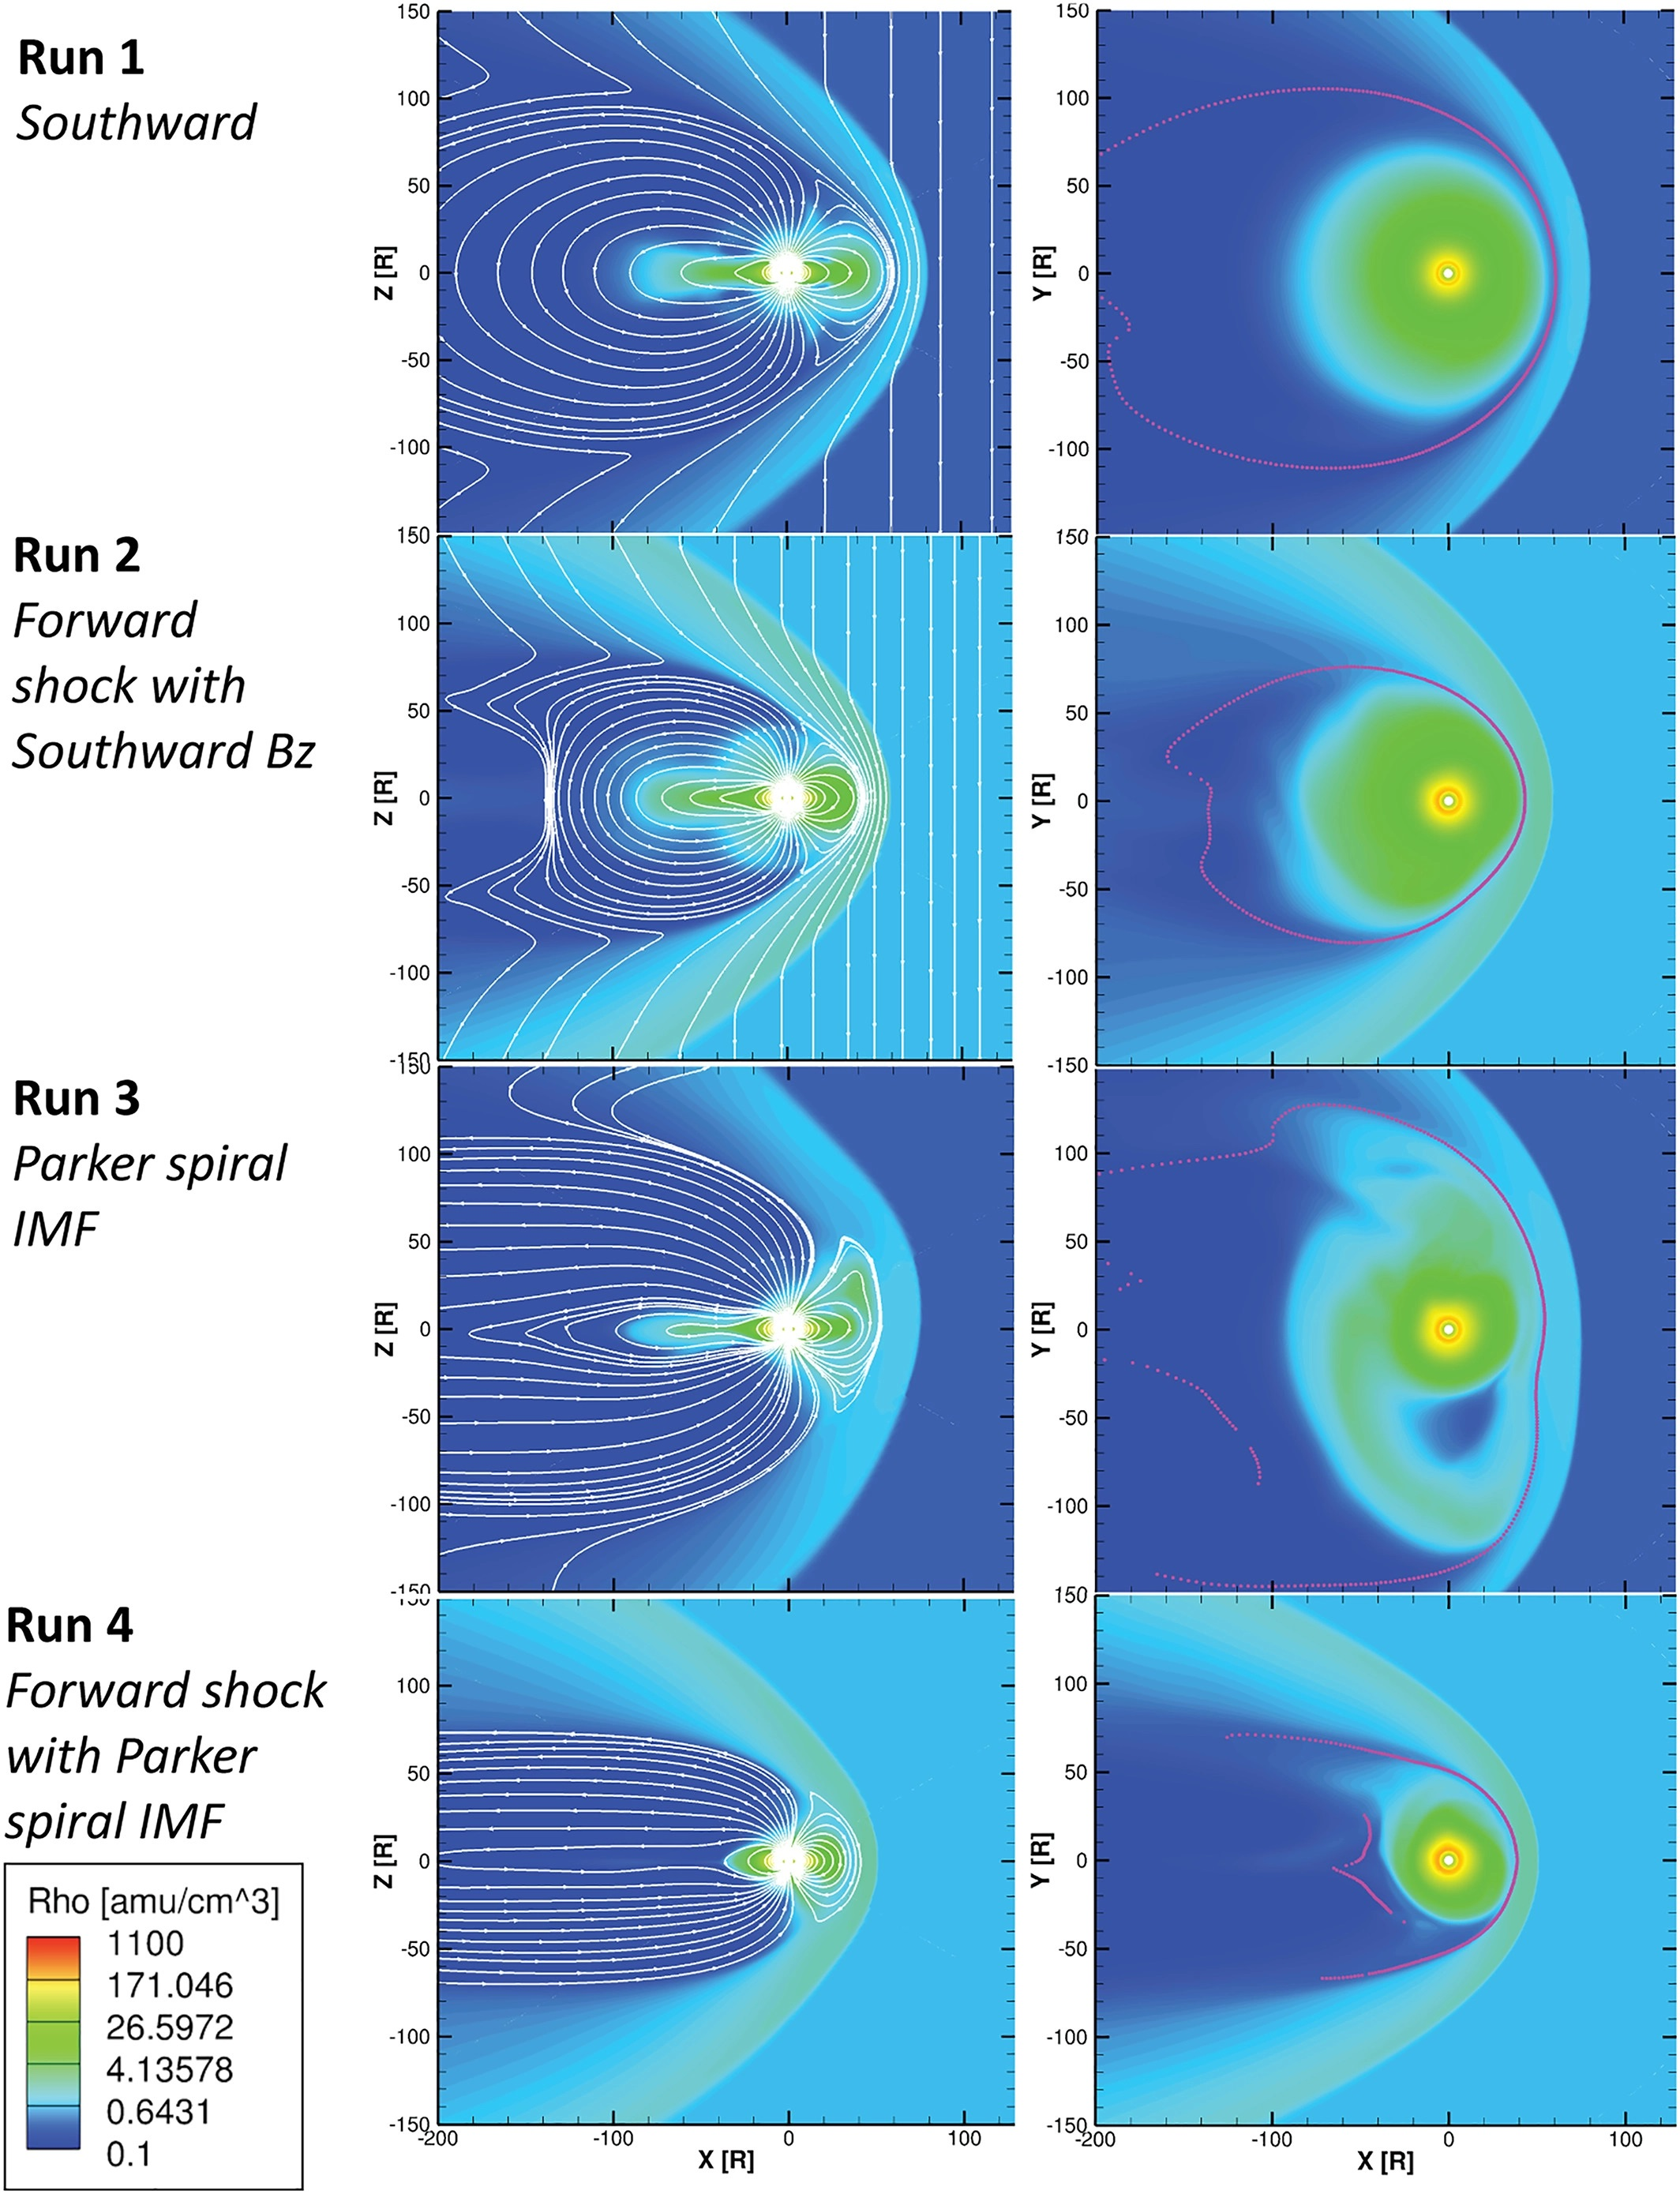
\includegraphics[width=0.8\textwidth]{images3/mhd-solarwind-upstream.jpg}
    \caption{The magnetospheric response to various solar wind conditions. Shown in the left column are plasma density contours in the noon-midnight meridian (XZ plane) with superimposed magnetic field lines in white. The right column shows the plasma density contours in the equatorial (XY) plane. The magneta dots are the identified equatorial crossings of the last closed field lines.}
    \label{fig:mhd-solarwind-upstream}
\end{figure}

In Figure \ref{fig:mhd-solarwind-upstream} we show the response of the magnetosphere from these four runs. Plotted in the left and right columns are contours of plasma mass density (log scale) in the meridional plane and equatorial plane, respectively, along with the equatorial footprints of the last closed field lines in a similar format as used for Figure 3. In the meridional ($Y = 0$) plane, we also superimpose magnetic field lines in white that illustrate the disk‐like configuration in the inner and middle magnetosphere, which is indicative of the presence of a strong current sheet and departure of the magnetospheric field from dipolar configuration, which is qualitatively consistent with in situ magnetic field measurements \cite{Khurana2001}. 

\subsection{Magnetospheric Response to IMF Rotation (Run 3: From Southward \texorpdfstring{$B_Z$}{Bz} to Spiral IMF With \texorpdfstring{$B_Y > 0$}{By>0}) }

When the IMF is turned from parallel to a spiral configuration, the magnetic shear across the dayside magnetopause increases such that magnetic reconnection occurs at the dayside magnetopause in the simulation resulting in the twisted dayside magnetic field lines as shown Figure \ref{fig:mhd-solarwind-upstream}, row 3. On the nightside, the equatorial footprints of the last closed field lines provide a good proxy for the reconnection X‐line, and we find that after turning the IMF to the Parker‐spiral configuration, the tail X‐line moves planetward. The tail X‐line location also exhibits a dawn‐dusk asymmetry, being located further from the planet on the duskside and closer to the planet on the dawnside, consistent with that inferred from observations \cite{Vogt2010a,Vogt2014,Woch2002a}. In addition to the planetward shift of the tail X‐line, turning the IMF also adds open magnetic flux to the magnetotail lobes, which can also be seen in later plots (Figure \ref{fig:mhd-solarwind-upstream}) where we show the open flux in the ionosphere, and the consequence of the addition of open field lines will be discussed in later sections. As open field lines are added to the tail lobes, the tail magnetic field becomes more stretched with a strong $B_X$ component, in contrast to the dipolar configuration under parallel IMF conditions (Run 1 as shown in row 1 of Figure \ref{fig:mhd-solarwind-upstream}). 

\subsection{Magnetospheric Response to Dynamic Pressure Enhancement (Runs 2 and 4)}

The forward shock introduced in Runs 2 and 4 corresponds to a dynamic pressure enhancement of a factor of $\sim$5 (from 0.053 to 0.258 nPa) with the plasma properties upstream and downstream of the shock taken such that the Rankine‐Hugoniot shock relations are satisfied. For Run 2 where the IMF is maintained in the parallel orientation that results in a closed magnetosphere, compression by the introduced forward shock causes the bow shock to move from $\sim$80 to $\sim$60 $R_J$ at the subsolar point, whereas the subsolar magnetopause moves from $\sim$60 to $\sim$40 $R_J$. In the case of an open magnetosphere (Run 4 where the IMF is in the spiral configuration), the bow shock moves from $\sim$75 to $\sim$50 $R_J$, whereas the magnetopause moves planetward from $\sim$50 to $\sim$40 $R_J$ at the subsolar point in response to the shock of the same magnitude as in Run 2. The compression due to the forward shock shrinks the magnetosphere in all directions, including the lobes and magnetospheric flanks. In both cases of the closed and open magnetosphere, the last closed field lines move planetward on the nightside. Run 4 shows the location of the X‐line for the shocked Parker‐spiral IMF, and it lies between 50 and 70 $R_J$ near midnight. Near the magnetopause flanks, the last closed field lines lie at a distance of ~$100$ $R_J$ from the planet. This creates a peculiar configuration of the magnetotail where the closed field lines extend to larger distances on the flanks than in the midnight sector, similar to that predicted for Saturn by \cite{Jia2012}.

\section{Response of the ionosphere to variations in the upstream conditions}

\begin{figure}
    \centering
    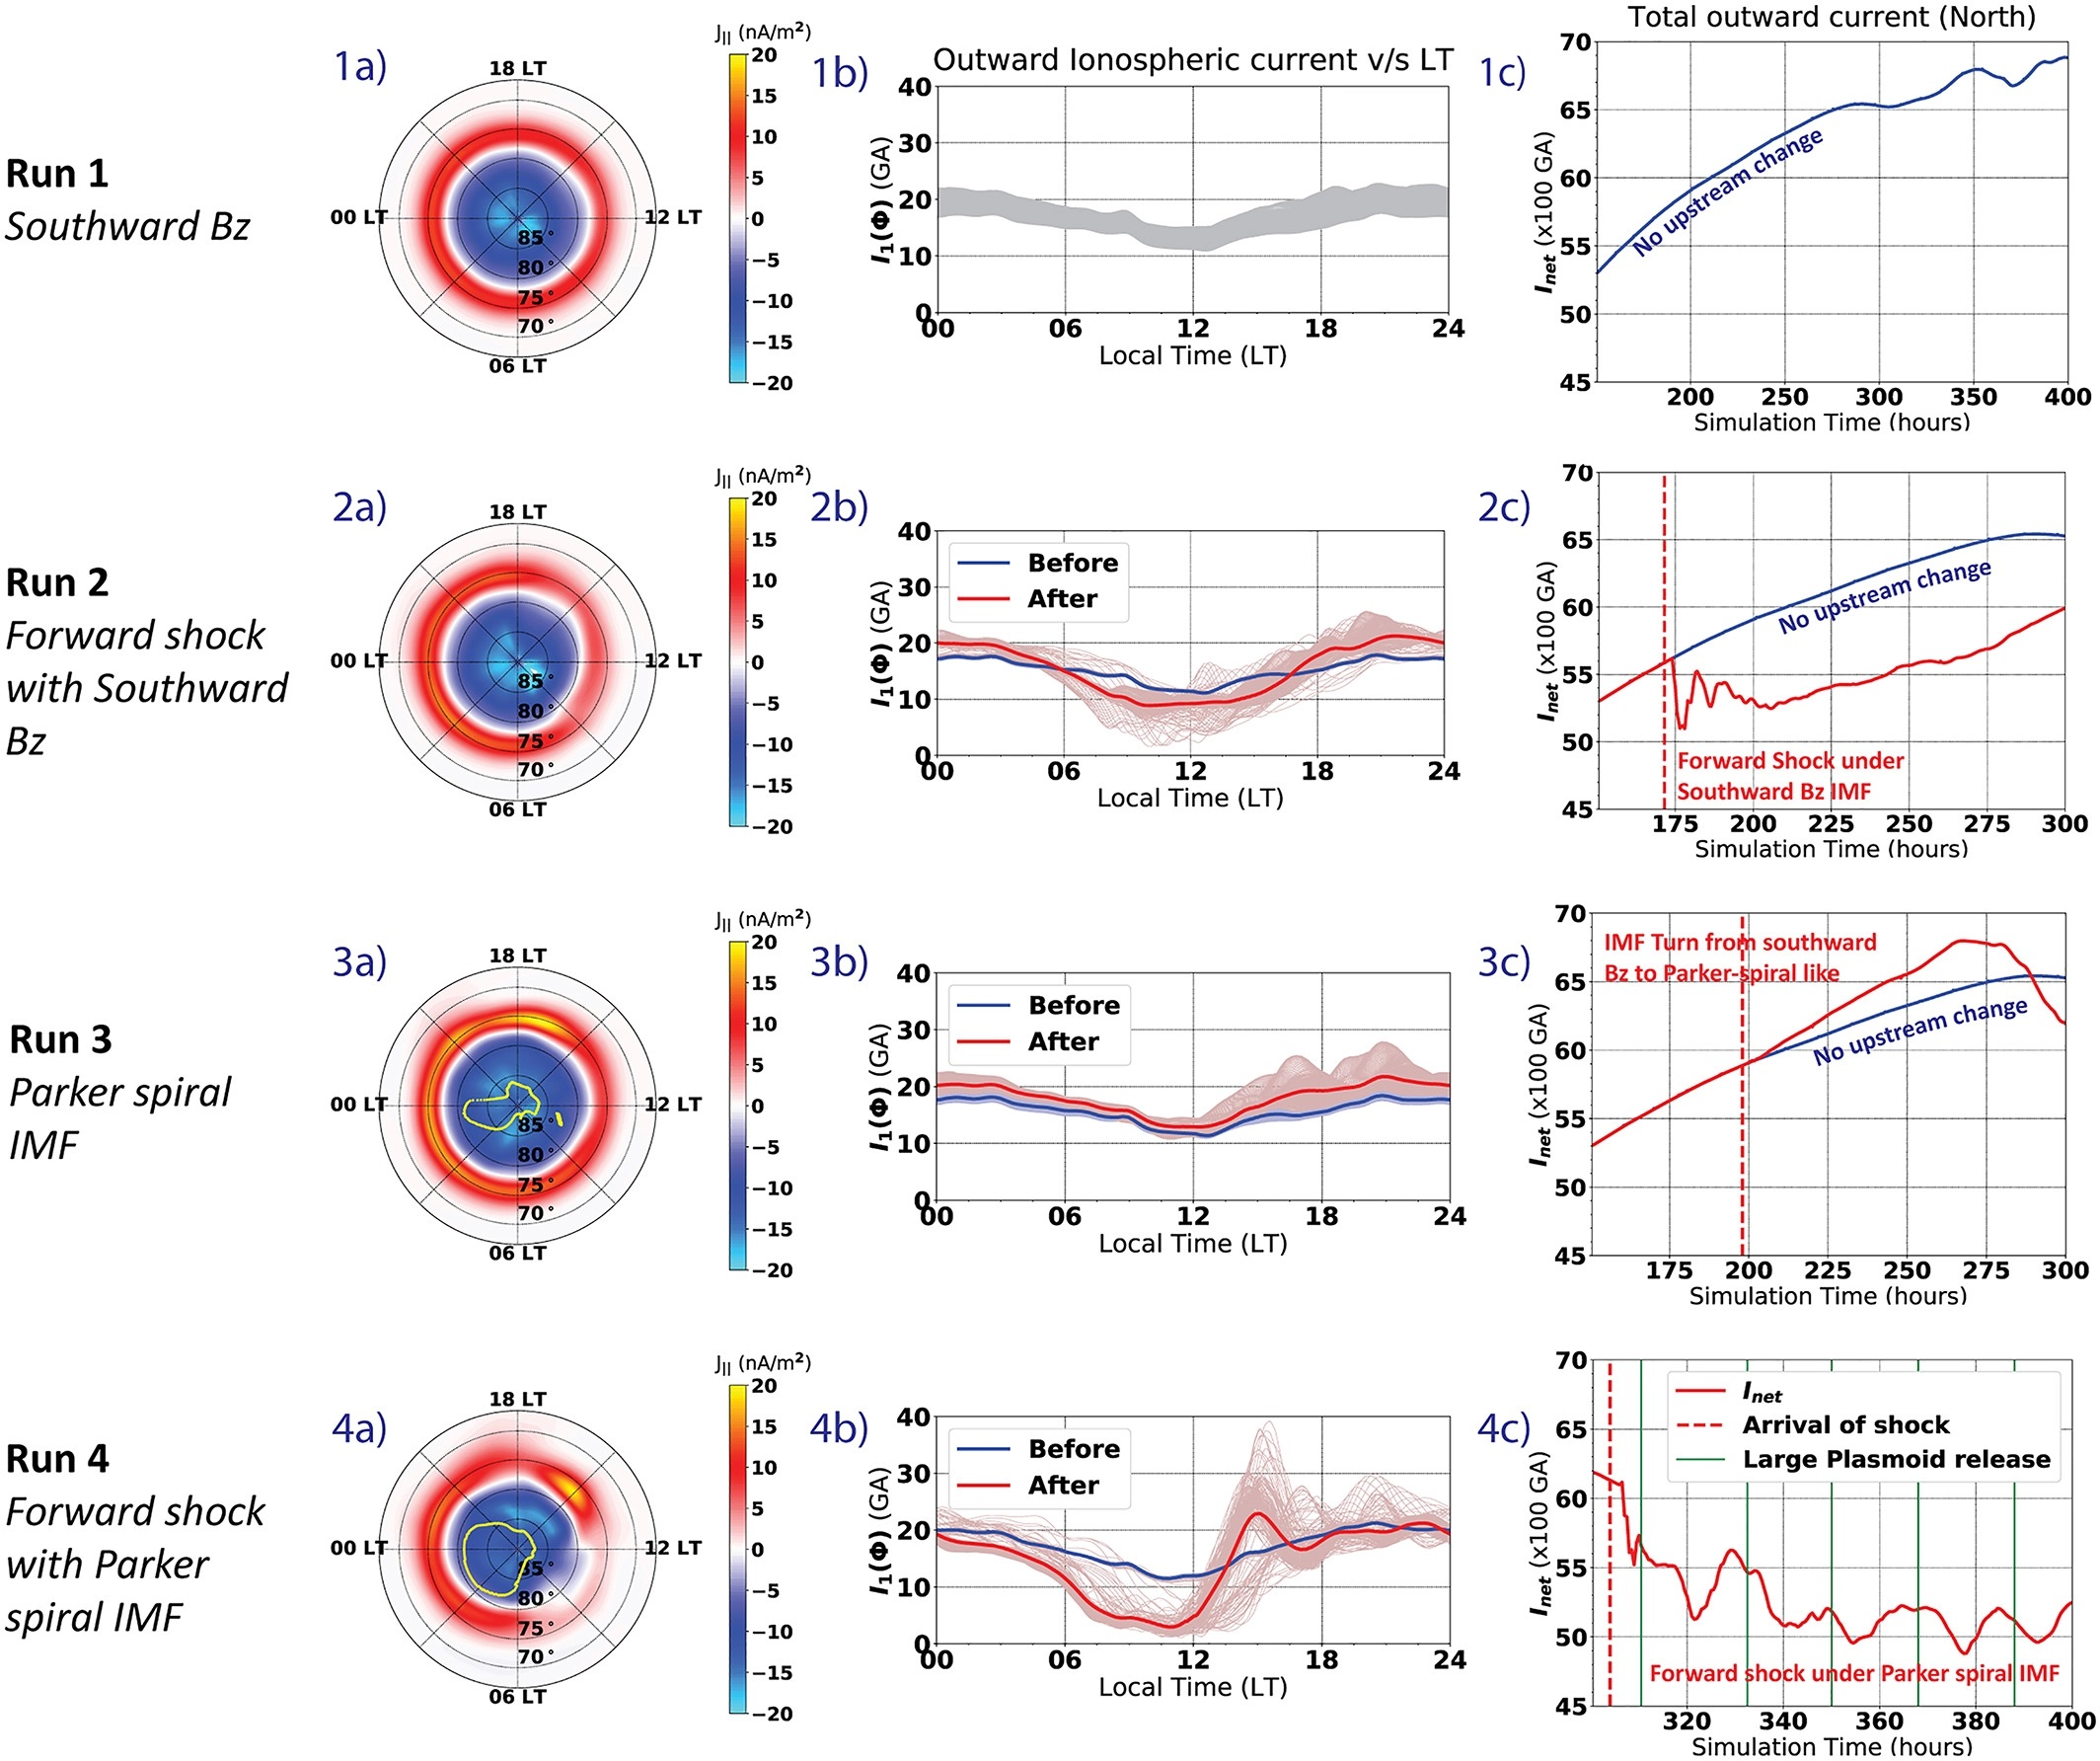
\includegraphics[width=0.9\textwidth]{images3/ionosphere-currents.jpg}
    \caption{Ionospheric response. Each row represents the ionospheric response to the four runs. The first column shows contours of radial current density at the ionosphere with positive values representing outward current. Yellow points are the extracted footprints at the open‐closed field line boundaries. In column 2 we show the latitude integrated outward current in the ionosphere as a function of local time. Each curve represents an instance in our simulation, with blue lines representing times before the upstream perturbation reaches the bow shock and red lines representing times after. In column 3 we show the total integrated outward current for all latitudes and local times as a function of simulation time. The blue curves in column 3 represent the variation of total outward current as a function of time for the closed magnetosphere under steady upstream conditions. The red curves represent the same quantity for the particular test case.}
    \label{fig:ionosphere-currents}
\end{figure}

Figure 8 shows the response of the ionosphere to changes in the different upstream conditions. The left column presents snapshots from each run showing the contours of the current density parallel to the magnetic field ($J_\parallel$). For the northern hemisphere shown here, positive values indicate outward currents and negative values indicate inward currents. The main feature of the current distribution is the circumpolar ring of outward currents centered at $\sim75^\circ$ latitude. Inside of (or poleward of) the ring are downward field‐aligned currents. The upward and downward currents are connected through the horizontal Pedersen currents in the ionosphere, and these currents together make up the corotation enforcement current system. 

Note that Ohm's law solver used in our model uses a spherical grid discretized at specific intervals in latitude and local time where each point can be identified by the indices $j$ and $i$ respectively. For a given simulation time $n$, we first calculate the net outward current (units of amperes) for a particular local time bin $i$ as,

\begin{equation}
    I_1^n \left(\phi\right)_i \approx \sum_{j=1}^{N_\theta} \left( \frac{|J_R| + J_R }{2} \right)_{i,j} \Delta s_{i,j}
\end{equation}

In this equation $J_{R_{i,j}}$ the radial current density at location $(i,j)$ and $\Delta s_{i,j}$ is the area of the spherical rectangle formed by the points $(i+1/2,j)$, $(i-1/2,j)$, $(i,j+1/2)$, and $(i,j-1/2)$. This parameter $I_1$ is plotted as a function of local time in column 2 of Figure 8. Each thin line represents the nth time of the simulation with a spacing of 0.5 hr. Thick blue or red lines represent the average value of I1 at a particular local time before and after changing the upstream conditions, respectively. As can be seen in column 2, the parameter $I_1$ is useful for revealing the local time‐dependent response of the outward currents, which are thought to be related to the emission intensity of Jupiter's main auroral oval. We then sum $I_1$ over all local times to obtain the net outward current (units of amperes) in one hemisphere at a particular time $n$ as - 

\begin{equation}
    I_{net}^n = \sum_i^{N_\phi} I_1^n(\phi)_i
\end{equation}

Here $N_\phi$ and $N_\theta$ are the number of grid cells in the azimuthal and meridional directions, respectively. In our simulations $N_\phi$ = 361 and $N_\theta$ = 181 for each hemisphere. The quantity $I_{net}$ represents the net outward current from one hemisphere and is plotted as a function of simulation time in Figure 8, column 3. The red vertical dashed line represents the time when the upstream perturbation reaches the subsolar bow shock. Blue curves in column 3 represent the trend expected if there was no change in upstream conditions (same the blue curve in Figure 8‐1c).

\subsection{Ionospheric response - Run 1 (Fixed upstream with parallel IMF)}

For the $\sim$400‐hr duration of Run 1 (Figures 8‐1a to 8‐1c), the magnetosphere remains largely closed due to the southward $B_Z$ IMF imposed at the upstream boundary. Figure 8‐1b shows that there is a persistent day‐night asymmetry present in the field‐aligned current distribution with outward currents stronger on the nightside than on the dayside. Figure 8‐1c also shows that the net outward current is steadily increasing with time (and at all local times/longitudes), despite the upstream conditions being constant. Initially, the rate of increase of the currents is almost linear, but with time the growth rate decreases and eventually the currents are seen to decrease. We believe that the growing trend of currents (with time scales of tens of hours), in the absence of any change in external conditions, is due to internal factors. As the magnetosphere builds more mass due to mass loading in the Io plasma torus, more torque is required from the ionosphere in order to force the magnetospheric plasma to corotate with the planet. Alternatively, consistent mass loading would increase the bend back of the magnetic field lines, which would increase magnetic field strength in the high‐latitude regions thereby increasing $J_\parallel$ in the ionosphere. Hence, prolonged mass loading in the absence of mass loss mechanisms, such as plasmoid release, would require an increase in the corotation enforcement currents. Indeed, we see that the ionospheric currents decrease only when a plasmoid is released (at around $t = 350$ hr), suggesting that with the release of mass to the magnetotail, the net strength of the corotation enforcement circuit is reduced. For comparisons with other runs, the curve showing the expected trend of the total current (i.e., Figure 8‐1c) is included in all sub-figures in the last column. 

\subsection{Ionospheric Response—Run 3 (Turning of the IMF to \texorpdfstring{$B_Y > 0$}{By>0}) }

In Run 3, the upstream plasma properties are kept the same as in Run 1, and a tangential discontinuity is introduced in the solar wind across which the IMF is rotated from southward to the Parker‐spiral configuration (with $B_Y$ > 0). As shown in Figure 8‐3a, reconnection at the magnetopause produces open magnetic field lines, and the open‐closed field line boundary (OCB; marked in yellow lines) starts to expand equatorward. At the time shown in this plot, which is roughly 75 hr after the IMF turning, the region of open field lines extends about a few degrees from the pole and the OCB lies at least 5$^\circ$ poleward of the main oval of outward currents. Similar to that in Run 1 (Figure 8‐1b), the outward currents in this run (Run 3) are stronger on the nightside than on the dayside (Figure 8‐3b) and a continuously increasing trend is seen for the net outward current (Figure 8‐3c). The red dashed line in Figure 8‐3c marks the time when the discontinuity reaches the subsolar bow shock, and we can see that the rate of increase of currents (shown by the red line) deviates from the curve expected if there were no change in the upstream conditions (shown in blue). Note that the only upstream change introduced in this run is the change in IMF clock angle. Therefore, the comparison between Run 1 and Run 3 indicates that a change in IMF orientation can have significant influences on the large‐scale current systems. The increasing trend of current, which now has a larger slope, eventually changes to a decreasing trend after the release of a plasmoid at $t = 270$ hr, consistent with the behavior seen in Run 1. 

\subsection{Ionospheric Response—Runs 2 and 4 (Dynamic Pressure Enhancement)}

In comparison to an IMF rotation, the response of the ionosphere to a forward shock, that is, a dynamic pressure enhancement, in the solar wind is more dramatic. In Runs 2 and 4, we have introduced a dynamic pressure enhancement (a factor of 5 larger than the background). First, we examine Run 2—that is, dynamic pressure enhancement under a closed magnetosphere (Figures 8‐2a–2c). In all our simulation runs, we find the nightside currents to be stronger than the dayside, and it can be seen from Figure 8‐2b that the introduction of a forward shock makes this asymmetry more pronounced; that is, the nightside currents get stronger whereas the dayside currents get weaker. Similar enhancement of the day‐night asymmetry has also been seen in the MHD model of \cite{Chane2017a}. Apart from the overall response, there are also noticeable local time‐dependent responses: Transient peaks in the outward current appear at specific local times. Our simulation predicts a minor enhancement on the nightside (10–20\% increase in total currents) and a large decrease in current on the dayside (between 10\% and 60\%). As a result, the net outward current ($I_{net}$) sharply decreases after the impingement of the shock. After 50 hours, the system recovers and an increasing trend of the net outward current is seen again. 

Our findings are consistent with previously published theoretical models 
\cite{Cowley2003a,Cowley2007,Southwood2001a}, which have predicted that a dynamic pressure enhancement, and subsequent compression of the magnetosphere, would lead to an increase in azimuthal velocity of the plasma as it conserves angular momentum. In theory, this should decrease the strength of the corotation enforcement current system on the dayside. Consistent with this prediction, we find an increase in angular velocity inside the magnetosphere on the dayside after the shock compression, which leads to much reduced outward field‐aligned currents in the dayside ionosphere. 

A similar behavior was also found for Run 4—that is, dynamic pressure enhancement with a Parker spiral IMF (Figures 8‐4a to 8‐4c). Due to the increase of magnetic flux reconnecting on the dayside and the release of plasmoids on the nightside (which serves to close previously opened tail lobes), we find a prominent region of open field lines in the polar region. We also find a very strong response of the ionospheric currents, with dayside currents drastically decreasing in strength (by 50–60\%), whereas the nightside currents appear almost unaffected (Figure 8‐4b). Consequently, the net outward current also decreases sharply after the dynamic pressure enhancement at $t = 310$ hours. A key difference between Figure 8‐4c and Figures 8‐1c, 8‐2c, and 8‐3c is that the time history of the total outward current did not recover back to the increasing trend after the dynamic pressure enhancement. This may be due to very frequent plasmoid releases in the magnetosphere after the shock compression. As seen in Runs 1 and 3, a decrease in the net outward current is well correlated with times at which a plasmoid is released. It is also noteworthy that the response of the ionosphere to the forward shock was stronger in Run 4 (open magnetosphere) than in Run 2 (closed magnetosphere). Apart from the IMF orientation, there is another difference between Runs 2 and 4: the phase of the magnetosphere in the Vasyliunas cycle. While Run 4 was started 30 hr after the release of a large plasmoid, Run 2 was initiated at a time when the magnetosphere was still in the process of accumulating mass with no prior plasmoid release. It is possible that the differences in the strength of the response may be due in part to the differences in the internal state of the magnetosphere, that is, depleted versus filled magnetosphere, rather than just the orientation of the external IMF. Clearly more work is needed to conclusively separate the internal and external influences. 

 

\section{Summary}

We have developed a new MHD model for Jupiter's magnetosphere using the BATSRUS MHD code. Time‐dependent simulations have been conducted with various upstream conditions to investigate how Jupiter's magnetosphere responds to changes in the solar wind and IMF properties. As model validation, we compare the modeled density, velocity, thermal pressure, magnetic field, and plasma $\beta$ extracted from multiple time steps and from simulation runs with different external conditions with available in situ observations and found generally good agreements. In particular, while our model underpredicts the plasma density (and pressure) in the inner magnetosphere ($<10 R_J$) due to potential reasons of grid resolution and/or the assumption of isotropic pressure in ideal MHD, our model results match very well the statistical results from observations outside of 10 $R_J$ in terms of plasma density, azimuthal velocity, and the magnetic field. Further, our model also captures the dawn‐dusk asymmetries in the thickness of the current sheet \cite{Khurana2005,Vogt2011a} as observed by the Galileo spacecraft, that is, thicker current sheet on the duskside compared to dawn. The locations of the magnetopause and bow shock in our model are also generally consistent with the predictions by the empirical models of \cite{Joy2002a}, although our simulated magnetopause is slightly smaller in size due to the lack of energetic particles in the MHD model. 

After creating a quasi‐steady state magnetosphere in the simulation, we introduce various types of changes in the upstream solar wind and IMF, such as an IMF rotation and a dynamic pressure enhancement under southward IMF and Parker spiral IMF conditions. We find that changing the IMF orientation from a southward (parallel) to Parker‐spiral like IMF creates open flux in the magnetosphere and thereby modifies the large‐scale magnetospheric configuration, but it alone has little effect on the corotation enforcement current system. However, in the cases where a forward shock is introduced in the solar wind, it has a significant impact on the global magnetosphere‐ionosphere system. In particular, all of our simulations show that there is an apparent asymmetry in the field‐aligned current intensity in the ionosphere between the dayside and the nightside, with more intense currents on the nightside. This day‐night asymmetry is further enhanced by the compression of the magnetosphere by a forward shock. In the simulation where a shock is introduced under Parker‐spiral IMF conditions (Run 4), a region of intense field‐aligned currents is present in the afternoon local time sector (16 LT; Figures 8‐4a and 8‐4b), which magnetically maps to a region in the middle magnetosphere containing vortical plasma flows created due to the interaction between the return flow from tail reconnection with the corotating plasma. Although the ionospheric currents respond to the forward shock in both simulations (Runs 2 and 4), the magnitude of the response is significantly different. In general, when the magnetosphere contains more open flux (Run 4) due to dayside reconnection, the response of the ionosphere is stronger. It should be noted that while these two runs use the same solar wind parameters with the only difference being the IMF orientation used, the magnetospheric states prior to the shock impact are quite different, which may contribute in part to the differences seen in the simulated response. Future work is needed in order to isolate these two effects, that is, preconditioning of the magnetosphere and the influence of the IMF orientation. 

Plasmoid release in the tail has long been suggested to be an important means of plasma transport, and signatures of plasmoids have indeed been found in various in situ observations in Jupiter's magnetotail. Our global simulations also show plasmoid formation and release due to reconnection in the magnetotail. The majority of plasmoids seen in our simulations appear to form initially on closed magnetic field lines, consistent with the picture proposed by \citeA{Vasyliunas1983a}. While differing in size, all the plasmoids produced in the simulations develop a complex magnetic topology as they evolve and propagate downtail. As an example, we have shown the time evolution of two plasmoids with different sizes and their mapping to the polar ionosphere. Our magnetic mapping results support the previous hypothesis that the complex morphology of tail plasmoids may be responsible for creating puzzling auroral features such as arcs and filaments \cite{Grodent2003a,McComas2007,Nichols2009a}. 

As a quantitative measure of the influence of the external driver on the global magnetospheric configuration, we have identified the OCB throughout our simulations by tracing 3D magnetic field lines. We have also calculated the total amount of open flux within the magnetosphere and examine the time evolution of the open flux in response to the changes imposed on the upstream parameters. For southward IMF, the magnetosphere has little to no open flux, as expected. As the IMF orientation is changed to a more realistic Parker spiral configuration, open magnetic flux starts to be added to the magnetosphere due to the dayside magnetopause reconnection and as such the OCB in the ionosphere starts to expand in size moving equatorward. In all the simulations present here, the OCB is found to be always located poleward by at least a few degrees of the main oval of upward field‐aligned currents associated with corotation breakdown. The total amount of open flux is found to peak around 200 GWb for typical Parker‐spiral IMF conditions, which is about a factor of 2 smaller than previously published estimates \cite{Vogt2011a}. There is a clear correlation between the reduction of open flux and the release of plasmoids in the tail, whose occurrence frequency appears to be affected by the solar wind convectional electric field with more frequent release under stronger driving. Based on the time rate of change of the open magnetic flux, we estimate the average potential drop associated with the dayside reconnection under nominal solar wind conditions to be approximately 280 kV, which is about a factor of 2 lower than previous estimates \cite{Masters2017}. 

In the present study we have assumed that Jupiter's internal magnetic field is an axisymmetric dipole. However, recent observations by Juno have revealed significant north‐south asymmetries in the internal magnetic field \cite{Connerney2018} due to the presence of large higher order moments. How the complex internal magnetic field influences the magnetosphere and its interaction with the ionosphere and the solar wind remains an outstanding question that needs to be addressed in future work. 